
\documentclass[a4paper,11pt]{article}
\usepackage[a4paper, margin=8em]{geometry}

% usa i pacchetti per la scrittura in italiano
\usepackage[french,italian]{babel}
\usepackage[T1]{fontenc}
\usepackage[utf8]{inputenc}
\frenchspacing 

% usa i pacchetti per la formattazione matematica
\usepackage{amsmath, amssymb, amsthm, amsfonts}

% usa altri pacchetti
\usepackage{gensymb}
\usepackage{hyperref}
\usepackage{standalone}

% imposta il titolo
\title{Appunti Fondamenti di Automatica}
\author{Luca Seggiani}
\date{2025}

% disegni
\usepackage{pgfplots}
\pgfplotsset{width=10cm,compat=1.9}

% imposta lo stile
% usa helvetica
\usepackage[scaled]{helvet}
% usa palatino
\usepackage{palatino}
% usa un font monospazio guardabile
\usepackage{lmodern}

% tikz in sans
\tikzset{every picture/.style={/utils/exec={\sffamily}}}

\renewcommand{\rmdefault}{ppl}
\renewcommand{\sfdefault}{phv}
\renewcommand{\ttdefault}{lmtt}

% circuiti
\usepackage{circuitikz}
\usetikzlibrary{babel}

% disponi il titolo
\makeatletter
\renewcommand{\maketitle} {
	\begin{center} 
		\begin{minipage}[t]{.8\textwidth}
			\textsf{\huge\bfseries \@title} 
		\end{minipage}%
		\begin{minipage}[t]{.2\textwidth}
			\raggedleft \vspace{-1.65em}
			\textsf{\small \@author} \vfill
			\textsf{\small \@date}
		\end{minipage}
		\par
	\end{center}

	\thispagestyle{empty}
	\pagestyle{fancy}
}
\makeatother

% disponi teoremi
\usepackage{tcolorbox}
\newtcolorbox[auto counter, number within=section]{theorem}[2][]{%
	colback=blue!10, 
	colframe=blue!40!black, 
	sharp corners=northwest,
	fonttitle=\sffamily\bfseries, 
	title=Teorema~\thetcbcounter: #2, 
	#1
}

% disponi definizioni
\newtcolorbox[auto counter, number within=section]{definition}[2][]{%
	colback=red!10,
	colframe=red!40!black,
	sharp corners=northwest,
	fonttitle=\sffamily\bfseries,
	title=Definizione~\thetcbcounter: #2,
	#1
}

% disponi problemi
\newtcolorbox[auto counter, number within=section]{problem}[2][]{%
	colback=green!10,
	colframe=green!40!black,
	sharp corners=northwest,
	fonttitle=\sffamily\bfseries,
	title=Problema~\thetcbcounter: #2,
	#1
}

% disponi codice
\usepackage{listings}
\usepackage[table]{xcolor}

\lstdefinestyle{codestyle}{
		backgroundcolor=\color{black!5}, 
		commentstyle=\color{codegreen},
		keywordstyle=\bfseries\color{magenta},
		numberstyle=\sffamily\tiny\color{black!60},
		stringstyle=\color{green!50!black},
		basicstyle=\ttfamily\footnotesize,
		breakatwhitespace=false,         
		breaklines=true,                 
		captionpos=b,                    
		keepspaces=true,                 
		numbers=left,                    
		numbersep=5pt,                  
		showspaces=false,                
		showstringspaces=false,
		showtabs=false,                  
		tabsize=2
}

\lstdefinestyle{shellstyle}{
		backgroundcolor=\color{black!5}, 
		basicstyle=\ttfamily\footnotesize\color{black}, 
		commentstyle=\color{black}, 
		keywordstyle=\color{black},
		numberstyle=\color{black!5},
		stringstyle=\color{black}, 
		showspaces=false,
		showstringspaces=false, 
		showtabs=false, 
		tabsize=2, 
		numbers=none, 
		breaklines=true
}

\lstdefinelanguage{javascript}{
	keywords={typeof, new, true, false, catch, function, return, null, catch, switch, var, if, in, while, do, else, case, break},
	keywordstyle=\color{blue}\bfseries,
	ndkeywords={class, export, boolean, throw, implements, import, this},
	ndkeywordstyle=\color{darkgray}\bfseries,
	identifierstyle=\color{black},
	sensitive=false,
	comment=[l]{//},
	morecomment=[s]{/*}{*/},
	commentstyle=\color{purple}\ttfamily,
	stringstyle=\color{red}\ttfamily,
	morestring=[b]',
	morestring=[b]"
}

% disponi sezioni
\usepackage{titlesec}

\titleformat{\section}
	{\sffamily\Large\bfseries} 
	{\thesection}{1em}{} 
\titleformat{\subsection}
	{\sffamily\large\bfseries}   
	{\thesubsection}{1em}{} 
\titleformat{\subsubsection}
	{\sffamily\normalsize\bfseries} 
	{\thesubsubsection}{1em}{}

% disponi alberi
\usepackage{forest}

\forestset{
	rectstyle/.style={
		for tree={rectangle,draw,font=\large\sffamily}
	},
	roundstyle/.style={
		for tree={circle,draw,font=\large}
	}
}

% disponi algoritmi
\usepackage{algorithm}
\usepackage{algorithmic}
\makeatletter
\renewcommand{\ALG@name}{Algoritmo}
\makeatother

% disponi numeri di pagina
\usepackage{fancyhdr}
\fancyhf{} 
\fancyfoot[L]{\sffamily{\thepage}}

\makeatletter
\fancyhead[L]{\raisebox{1ex}[0pt][0pt]{\sffamily{\@title \ \@date}}} 
\fancyhead[R]{\raisebox{1ex}[0pt][0pt]{\sffamily{\@author}}}
\makeatother

\begin{document}

% sezione (data)
\section{Lezione del 09-04-25}

% stili pagina
\thispagestyle{empty}
\pagestyle{fancy}

% testo
\subsection{Diagrammi di Bode}
I diagrammi di Bode sono di 2 tipi:
\begin{enumerate}
	\item Il \textbf{diagramma di modulo} (o ampiezza): rappresenta il modulo di $G(j\omega)$ al variare della pulsazione $\omega$.
		Abbiamo quindi $|G(j \omega)|$ alle ordinate e $\omega$ alle ascisse, espresse in scala logaritmica.
		Il modulo si misura in deciBel (dB), già in scala logaritmica, mentre per la pulsazione $\omega$ si usa la scala logaritmica in base 10.
		Notiamo che il decibel è un \textbf{unità di misura relativa}: si interpreta come il rapporto fra due \textit{potenze}, espresso in scala logaritmica, dove per la seconda grandezza, detta \textbf{valore di riferimento}, assumiamo 1:
		$$
		\mathrm{dB} = 10 \cdot \log_{10} \left( \frac{P}{P_{ref}} \right) =  10 \cdot \log_{10} \left( \frac{P}{1} \right)
		$$
		Abbiamo quindi che il rapporto fra valore assoluto di ampiezza e il valore in decibel è:
		$$
		x_{dB} = 20 \log_{10}(|x|)
		$$

		Il 20 compare per via del fatto che consideriamo \textit{ampiezze}, mentre il decibel esprime rapporti fra \textit{potenze}.
	Abbiamo che la relazione fra ampiezza $A$ e potenza $P$ è quadratica:
	$$
	A^2 \propto P
	$$
	per cui si vuole calcolare effettivamente:
	$$
	\mathrm{dB} = 10 \cdot \log_{10} \left( \frac{P}{P_{ref}} \right) = 10 \cdot \log_{10} \left( \frac{A^2}{A_{ref}^2} \right) = 10 \cdot \log_{10} \left( \left( \frac{A}{A_{ref}} \right)^2 \right)
	$$
	$$
	= 10 \cdot 2 \cdot \log_{10} \left( \frac{A}{A_{ref}} \right) = 20 \cdot \log_{10} \left( \frac{A}{A_{ref}} \right)
	$$
	assunto $A_{ref} = 1$ come da ipotesi si ottiene la stessa formula di prima.

	\item Il \textbf{diagramma di fase:} rappresenta la fase di $G(j\omega)$ al variare della pulsazione $\omega$.
		Abbiamo quindi $\angle G(j \omega)$ alle ordinate e $\omega$ alle ascisse, la prima in scala lineare e la seconda nella stessa scala logaritmica in base 10 di prima.
\end{enumerate}

\subsubsection{Ascisse}
Abbiamo quindi che sulle \textbf{ascisse} abbiamo sempre la \textit{pulsazione} (rad/s) o \textit{frequenza} (Hz), che non sono esattamente uguali ma sono fra di loro direttamente proporzionali per un fattore di $2\pi$:
$$
f = \frac{\omega}{2\pi}
$$
Queste sono espresse in scala logaritmica, e troviamo quindi i seguenti intervalli relativi:
\begin{itemize}
	\item \textbf{Decade:} è la distanza in scala logaritmica tra numeri il cui raporto è 10;
	\item \textbf{Ottava:} è la distanza in scala logaritmica tra numeri il cui rapporto è 2.
\end{itemize}

\subsubsection{Ordinate}
Alle \textbf{ordinate} manteniamo invece, nel caso di un diagramma di modulo, lo spettro di ampiezza in unità logaritmiche (dB).
Abbiamo quindi che 0 dB equivalgono al valore di riferimento, che abbiamo detto è 1, mentre tutti gli altri valori si convertono usando la formula:
$$
\text{(decibel)} \quad 20 \log_{10}(10^\alpha) = 20 \cdot \alpha \quad \text{(scala logaritmica)}
$$

Nel caso di diagrammi di fase, invece, abiamo la fase in scala lineare, misurata in \textit{radianti} (rad) o in \textit{gradi} ($\circ$).

\par\medskip

Notiamo infine che il \textit{modulo} è una funzione \textbf{pari}:
$$
|G(j \omega)| = |G(-j \omega)|
$$
mentre la \textit{fase} è una funzione \textbf{dispari}:
$$
\angle G(j \omega) = - \angle G(-j \omega)
$$

\subsubsection{Proprietà dei diagrammi di Bode}
Abbiamo quindi che i diagrammi di Bode sono molto comodi per avere rappresentazioni dettagliate di grandezze che variano in campi notevolmente estese.

Notiamo le due proprietà
\begin{enumerate}
	\item 
I diagrammi di Bode di sistemi in cascata si ottengono come somma dei diagrammi di Bode dei singoli sottoinsiemi.
Questo perchè 2 sistemi in cascata con trasferimento $G_1(s)$ e $G_2(s)$ hanno trasferimento complessivo:
$$
G_{eq}(s) = G_1(s) \cdot G_2(s)
$$
ma come sappiamo la il logaritmo di un prodotto equivale alla somma dei logaritmi, ergo:
$$
\log \left( G_1(s) \cdot G_2(s) \right) = \log \left( G_1(s) \right) + \log \left( G_2(s) \right)
$$
da cui la tesi. \qed

	\item
I diagrammi di Bode di una funzione in forma fattorizzata si ottengono come somma dei diagrammi elementari dei singoli fattori, sempre dalla stessa proprietà di cui sopra.
\end{enumerate}

Queste considerazioni spiegano il perché delle scale logaritmiche: infatti se indichiamo le grandezze:
$$
a = |a| e^{j \angle a}, \quad b = |b| e^{j \angle b}
$$
e prendiamo il prodotto, si ha che:
$$
a \cdot b = |a| |b| e^{j (\angle a + \angle b)}
$$
cioè gli angoli già si sommano in in scala lineare, mentre adottando la scala logaritmica per le ampiezze si ha:
$$
\log \left( |a||b| \right) = \log \left( |a| \right) + \log \left( |b| \right)
$$

\subsection{Forme fattorizzate}
Vediamo quindi nel dettaglio come ricavare i diagrammi di Bode (quindi ampiezza e argomento) di funzioni in forma fattorizzata.
Avremo che in questo caso la funzione di trasferimento ha l'aspetto:
\begin{equation}
G(s) = \frac{\prod_{i=1}^m(s - z_i)}{\prod_{i=1}^n(s - p_i)}
\end{equation}
con \textbf{zeri} al \textit{numeratore} e \textbf{poli} al \textit{denominatore}.

Quello che fa il logaritmo è semplificare questa configurazione, in quanto i prodotti diventano somme e i rapporti diventano sottrazioni.
Allora varrà che:
\begin{itemize}
	\item Il valore in dB del modulo sarà dato dalla differenza tra le sommatorie dei valori in dB dei moduli dei fattori del numeratore e dei fattori del denominatore;
	\item L'argomento sarà dato dalla differenza tra le sommatorie degli argomenti dei fattori del numeratore e del denominatore.
\end{itemize}

Avremo quindi che $G(s)$ con $s = j\omega$, cioè sistema asintoticamente stabile (si trascura la risposta transiente), dà:
$$
G(j \omega) = \frac{K_B}{(j \omega)^h} 
\cdot
\frac{ \prod_{i}^{m - u} (1 \pm j \omega T_{z_i}) }{ \prod_{i = 1}^{n - h - r} (1 \pm j \omega T_{p_i}) } 
\cdot
\frac{ \prod_{i = 1}^u \left( 1 \pm j \omega \frac{ 2 \xi_{z_i} }{\omega_{0_{z_i}}} - \frac{\omega^2}{\omega_{0_{z_i}}^2} \right) }{ \prod_{i = 1}^r \left( 1 \pm j \omega \frac{ 2 \xi_{p_i} }{\omega_{0_{p_i}}} - \frac{\omega^2}{\omega_{0_{p_i}}^2} \right) }
$$
dove si è preso:
\begin{itemize}
	\item $h$: numero di poli all'origine, detto anche \textit{tipo} del sistema; 
	\item $K_B$: guadagno di Bode;
	\item $m$: numero di zeri;
	\item $h$: numero di poli;
	\item $u$: numero di zeri complessi coniugati;
	\item $r$: numero di poli complessi coniugati.
\end{itemize}

Quindi il primo termine rappresenterà il guadagno statico di Bode, il secondo termine rappresenterà gli zeri e i poli \textit{semplici}, e il terzo termine rappresentera gli zeri e i poli complessi coniugati.

Questa, notiamo, è effettivamente la forma di Bode della (1) (che è una forma di Evans). 

Vediamo quindi di applicare quanto avevamo detto al caso con \textit{soli} \textbf{poli semplici}.
\begin{itemize}
	\item 
Il modulo logaritmico sarà:
$$
\log \left( G(j \omega) \right) = \sum_{i = 1}^{m} \log \left( |1 \pm j \omega T_{z_i}| \right) - \sum_{i = 1}^{n} \log \left( |1 \pm j \omega T_{p_i}| \right)
$$
cioè si prendono i logaritmi dei moduli degli zeri meno i logaritmi dei moduli dei poli. 

\item 
La fase sarà:
$$
\angle G(j \omega) = \sum_{i = 1}^{m} \log \left( \angle \left( 1 \pm j \omega T_{z_i} \right) \right) - \sum_{i = 1}^{n} \log \left( \angle \left( 1 \pm j \omega T_{p_i} \right) \right)
$$
cioè si prendono i logaritmi delle fasi degli zeri meno i logaritmi delle fasi dei poli. 
\end{itemize}

\par\bigskip

Da qui in poi vedremo qunidi come tracciare i diagrammi di Bode di alcuni sistemi comuni.

\subsubsection{Guadagno costante}
Prendiamo la funzione di trasferimento a guadagno costante:
$$
G(s) = K
$$
Questa si limiterà a prendere l'ingresso e restituirlo scalato di $K$ in uscita.

La funzione di risposta armonica si calcola semplicemente ponendo $s = j \omega$, che in questo caso non ha effetto:
$$
G(j \omega) = K 
$$
e quindi si ha il modulo:
$$
|G(j \omega)| = |K|
$$
e la fase:
$$
\angle G(j \omega) = 0 
$$

Per tracciare il modulo, ricordiamo che vogliamo trovare $k_{dB}$:
$$
K_{dB} = 20 \log_{10}(|K|) 
$$

Possiamo compilare una tabella dei valori tipici in dB di moduli di funzione:
\begin{table}[H]
	\center \rowcolors{2}{white}{black!10}
	\begin{tabular} { c | c }
		$|K|$ & $K_{dB}$ \\ 
		\hline
		$\sqrt{2}$ & $3$ dB \\
		$2$ & $6$ dB \\
		$5$ & $14$ dB \\
		$20$ & $26$ dB \\
		$50$ & $36$ dB 
	\end{tabular}
\end{table}
e notiamo inoltre di poter sfruttare le proprietà dei logaritmi per dire:
$$
20 \log_{10}(|K|) = K_{dB} \implies 20 \log_{10}\left(\frac{1}{|K|}\right) = - K_{dB}
$$

Prendiamo quindi $K = 5$, e troviamo quindi che il valore in decibel dovrà essere $14$ dB.

\par\medskip

\noindent
\begin{minipage}{\textwidth}
Potremo allora tracciare il grafico del modulo in decibel:
\begin{center}
	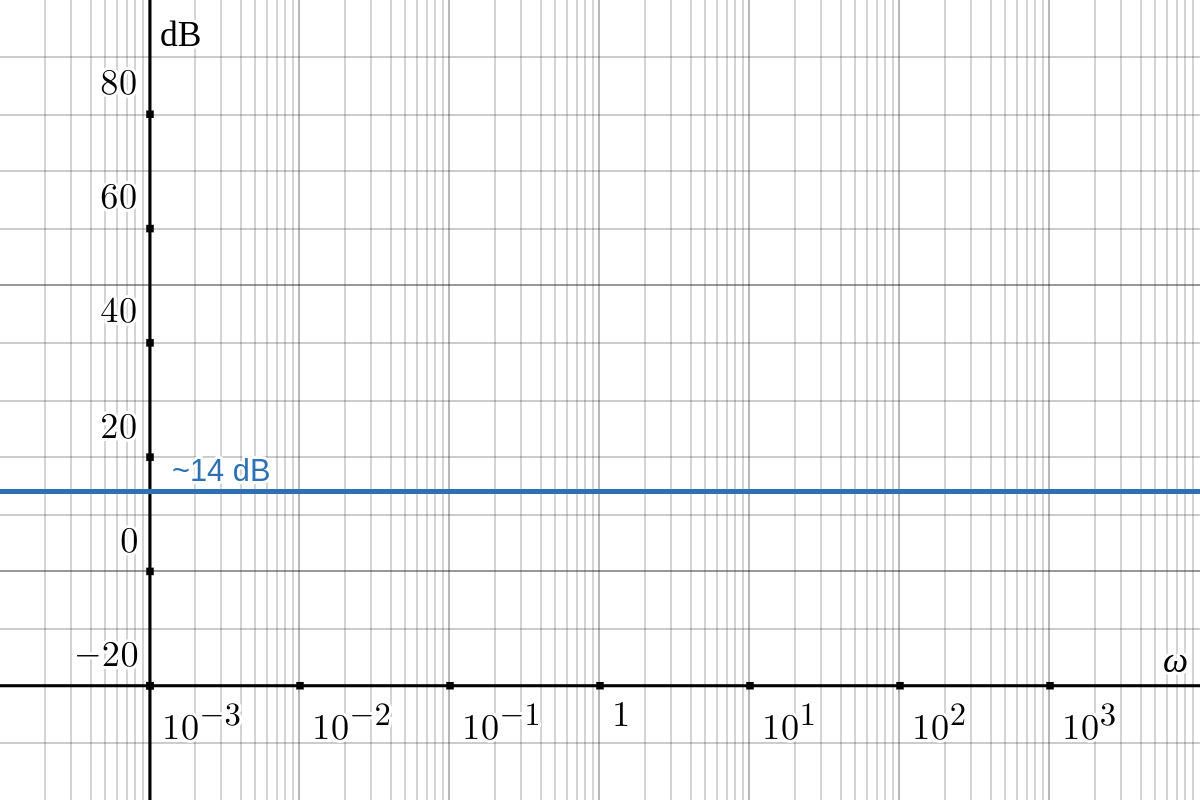
\includegraphics[scale=0.3]{../figures/costant_bode/mod.png}
\end{center}
\end{minipage}

\par\medskip

Per quanto riguarda la fase, il grafico è invece banale:
\begin{center}
	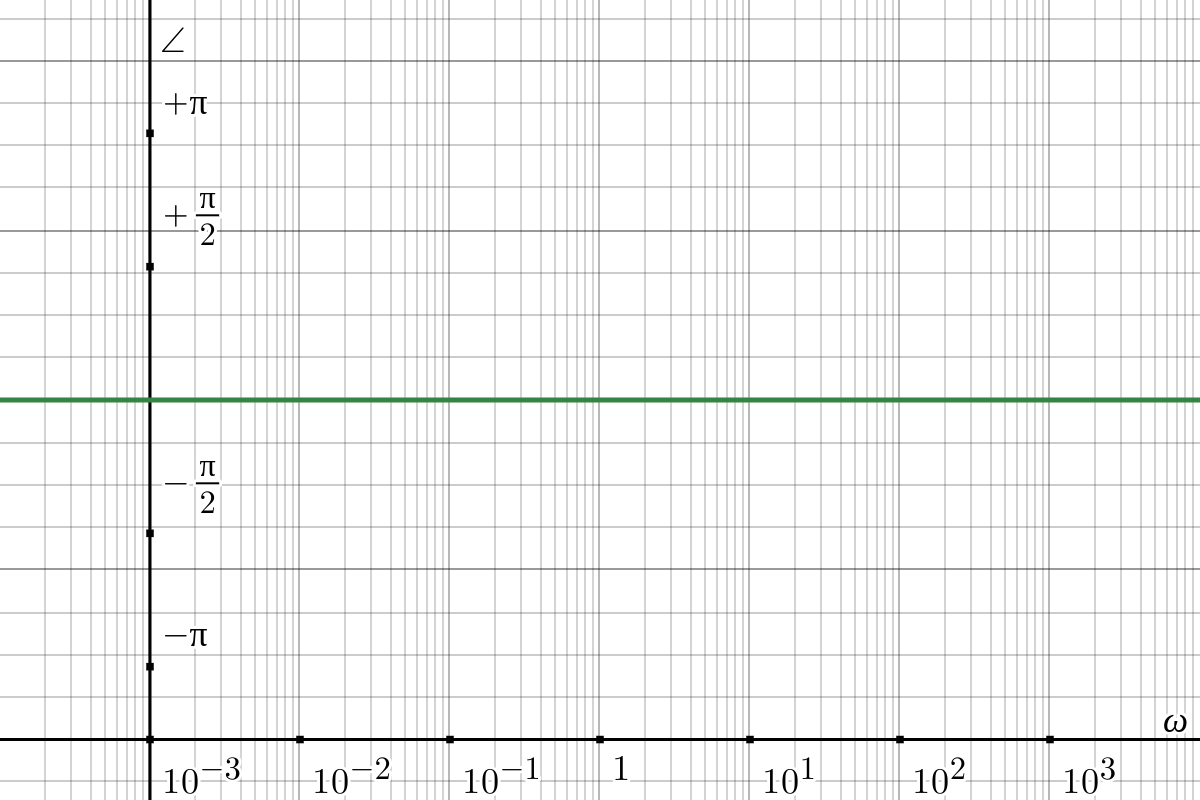
\includegraphics[scale=0.3]{../figures/costant_bode/phase.png}
\end{center}
in quanto corrisponde alla retta di sfasamento 0.

\subsection{Poli reali: integratori}
Vediamo la classe di risposte in frequenza date dai sistemi con poli reali semplici.

\subsubsection{Poli all'origine}
Ricordiamo che il polo all'origine rappresenta nel dominio di Laplace l'\textbf{integratore}:
$$
\frac{1}{s}
$$

Considereremo quindi funzioni di trasferimento del tipo:
$$
G(s) = \frac{1}{s} \implies G(j \omega) = \frac{1}{j\omega}
$$
passando alla risposta armonica.

Il modulo in questo caso sarà:
$$
|G(j\omega)| = \frac{1}{\omega} 
$$
che notiamo in logaritmo (dB) dà:
$$
20 \log_{10} \left( \omega^{-1} \right) = - 20 \log_{10} (\omega)
$$

\par\medskip

\noindent
\begin{minipage}{\textwidth}
cioè si ottiene una retta nel diagramma del modulo logaritmico che passa per $\omega =1$ con modulo 0 dB e pendenza -20 dB/dec (cioè -6 dB/oct):
\begin{center}
	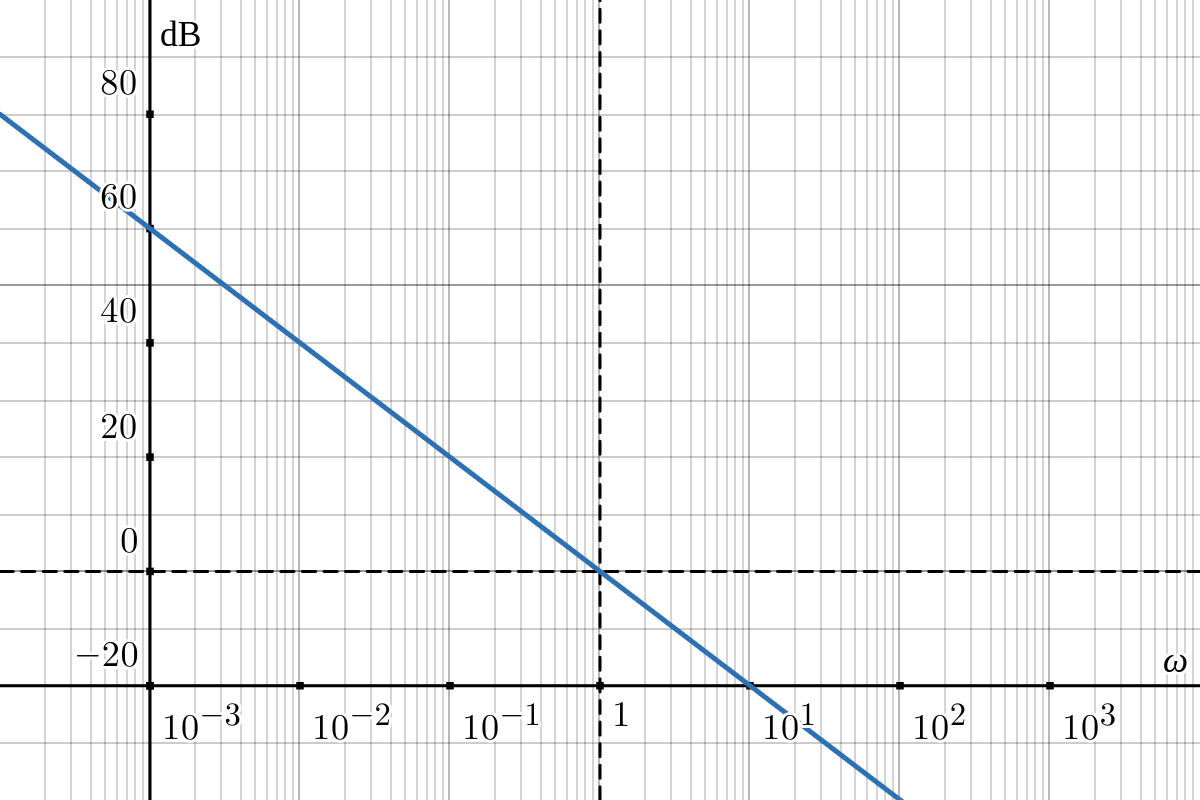
\includegraphics[scale=0.3]{../figures/integrator_bode/mod.png}
\end{center}
\end{minipage}

\par\medskip

Per quanto riguarda la fase, invece, avremo scostamento costante:
$$
\angle G(j \omega) = - \frac{\pi}{2}
$$

\par\medskip

\noindent
\begin{minipage}{\textwidth}
da cui il grafico:
\begin{center}
	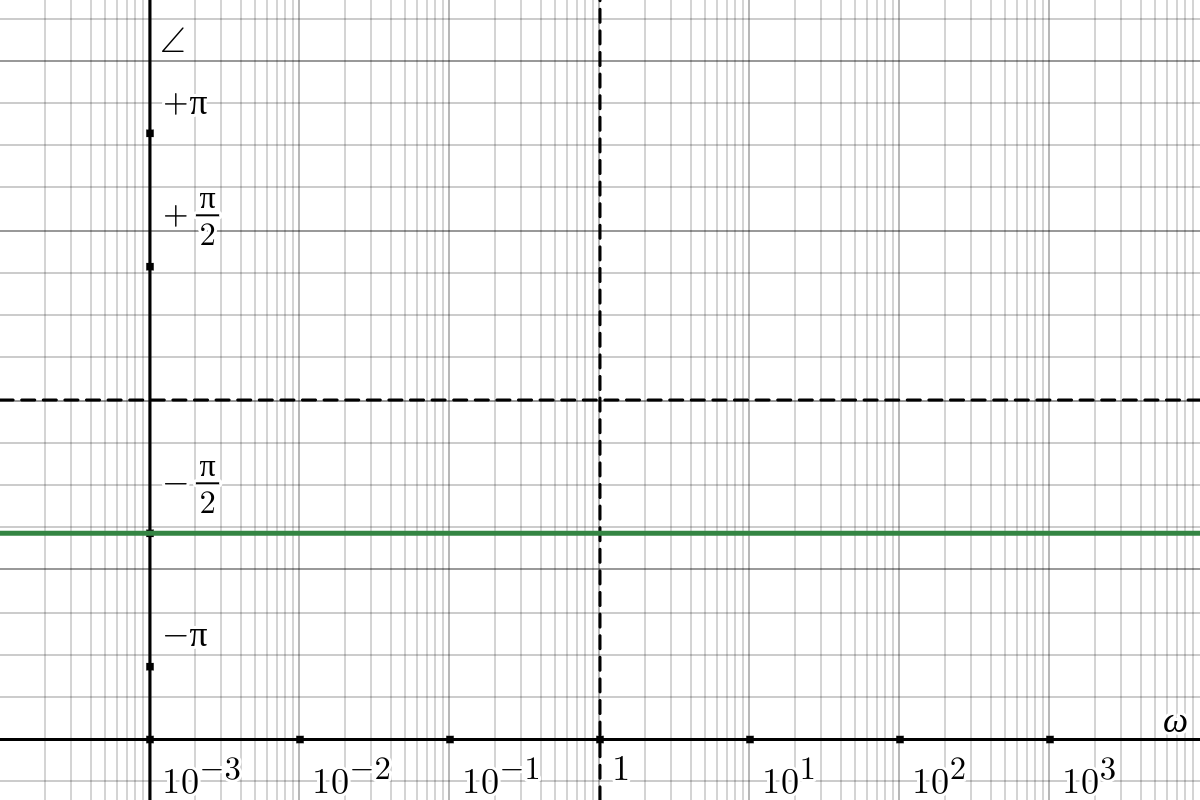
\includegraphics[scale=0.3]{../figures/integrator_bode/phase.png}
\end{center}
\end{minipage}

\par\medskip

\subsubsection{Poli reali}
Prendiamo quindi la funzione con un solo polo reale in $-\frac{1}{\tau}$, che notiamo non essere altro che l'esempio precedente col polo scostato verso il lato reale negativo del piano complesso:
$$
G(s) = \frac{1}{1 + \tau s} 
$$
da cui la risposta armonica:
$$
G(j \omega) = \frac{1}{1 + j \omega \tau}
$$

Il modulo è quindi:
$$
|G(j \omega)| = \frac{1}{\sqrt{1 + \omega^2 \tau^2}}
$$

Questa funzione non è immediata da tracciare.
Vediamo di trovarne un approssimazione \textit{per rette}.
Distinguiamo quindi due situazioni attorno al cosiddetto \textbf{punto critico}, cioè il punto $\omega = 1$:
\begin{itemize}
	\item $\omega^2 \tau^2 << 1$, si ha:
		$$
		|G(j\omega)|_{dB} \approx 0 \, \mathrm{dB}
		$$
		cioè una costante a 0 dB di guadagno;
	\item $\omega^2 \tau^2 >> 1$, si ha, trascurando $1$:
		$$
		|G(j \omega)|_{dB} = 20 \log_{10} \left( \frac{1}{\omega \tau} \right) =
		20 \log \left( \frac{1}{\tau} \right) - 20 \log \left( \omega \right)
		$$
		che per $\tau = 1$ dà una retta con pendenza -20 dB/dec (cioè -6 db/oct).
\end{itemize}

\par\medskip

\noindent
\begin{minipage}{\textwidth}
Tracciamo quindi il grafico approssimato (sotto al quale si è tracciato il grafico esatto):
\begin{center}
	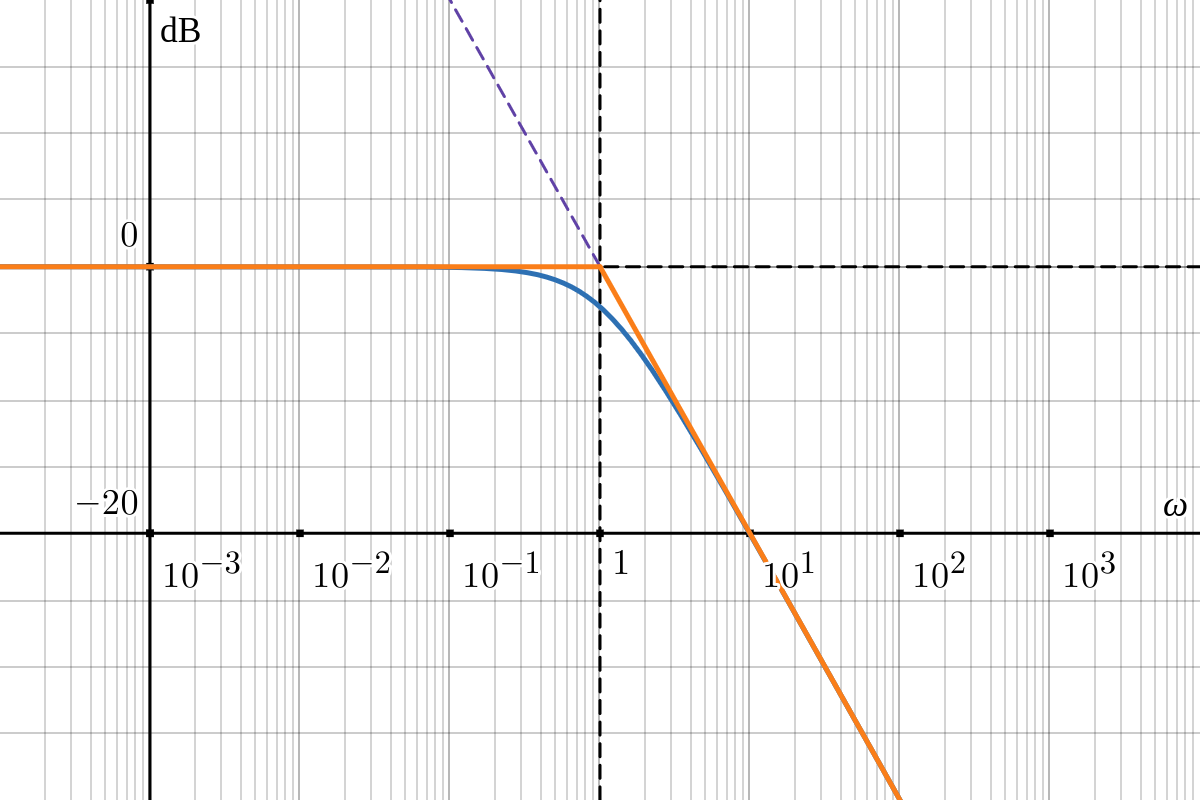
\includegraphics[scale=0.3]{../figures/lowpass_bode/mod.png}
\end{center}
\end{minipage}

\par\medskip

Dove si nota il decadimento al di sopra di $\omega = 1$ è lo stesso del caso del polo all'origine, e anzi spostare il polo verso la parte reale negativa ha il solo effetto di "troncare" la retta a una certa frequenza angolare $\omega= \frac{1}{\tau}$.

\par\smallskip

Ci potrebbe interessare valutare l'errore in $\omega = 1$.
Dalla nostra stima avevamo preso 0 dB, mentre sostituendo nella formula del modulo si ha:
$$
|G(j \cdot 1)| = \frac{1}{\sqrt{1 + \tau^2}}
$$
Ad esempio, preso $\tau = 1$ si ha $|G(j \cdot 1)| = \frac{1}{\sqrt{2}}$, che sappiamo valere -3 dB, per un errore complessivo di 3 dB.

\par\smallskip

Per quanto riguarda la fase potremmo invece dire:
$$
\angle G(j \omega) = - \tan^{-1} \left( \omega \tau \right)
$$
che potremo approssimare in:
\[
	\begin{cases}
		\omega \tau << 1 \implies \angle G(j\omega) \approx 0^\circ \\ 	
		\omega \tau >> 1 \implies \angle G(j\omega) \approx -90^\circ \\ 	
		\omega \tau = 1 \implies \angle G(j\omega) = -45^\circ \\ 	
	\end{cases}
\]
preso $\tau > 0$, cioè il caso con polo stabile.

\par\medskip

\noindent
\begin{minipage}{\textwidth}
Approssimiamo quindi questa funzione prendendo le rette a $0^\circ$ e $-90^\circ$, interpolate da una retta passante da $-45^\circ$ a $\omega = 1$:
\begin{center}
	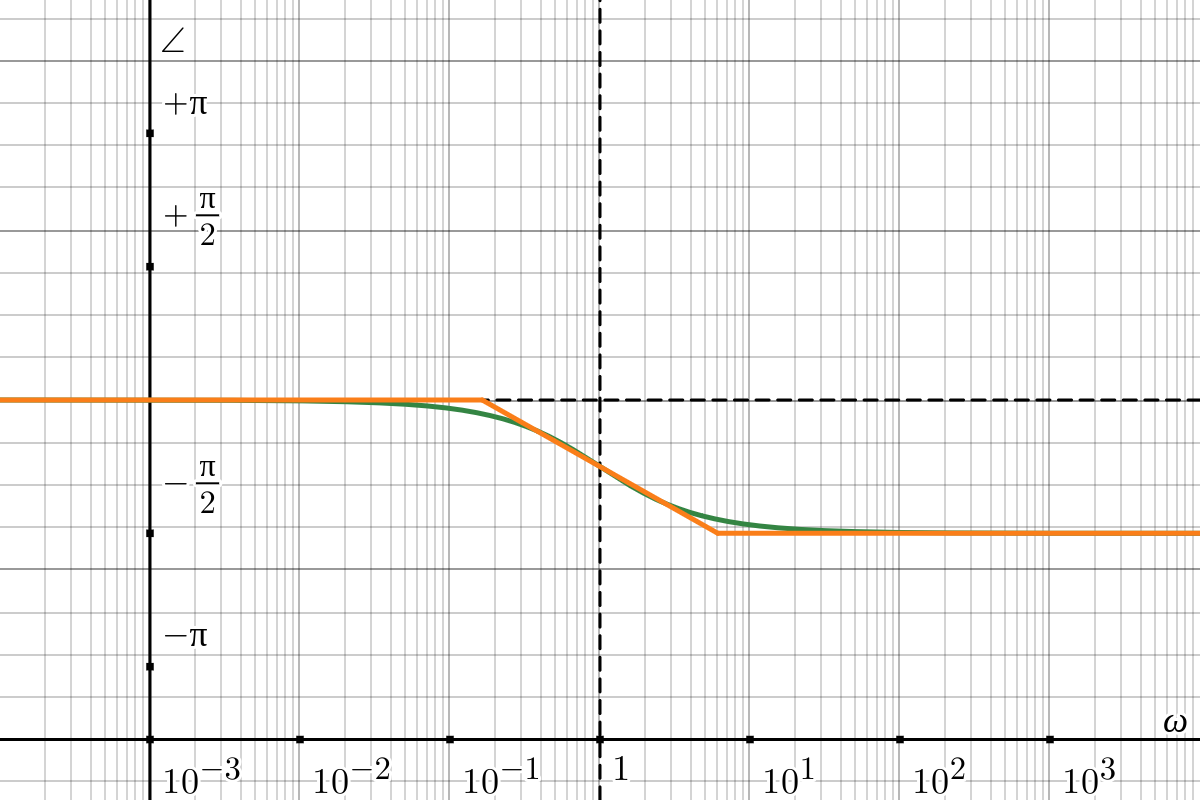
\includegraphics[scale=0.3]{../figures/lowpass_bode/phase.png}
\end{center}
\end{minipage}

\par\medskip

Notiamo un fatto particolare: nessuno ci nega, avendo trascurato le risposte transienti, di prendere il polo instabile in $1$, cioè quello dato da $\tau = -1$.

\par\medskip

\noindent
\begin{minipage}{\textwidth}
In questo caso nulla cambia riguardo alla risposta in modulo, mentre la risposta in fase cambia di segno, cioè si ha:
\begin{center}
	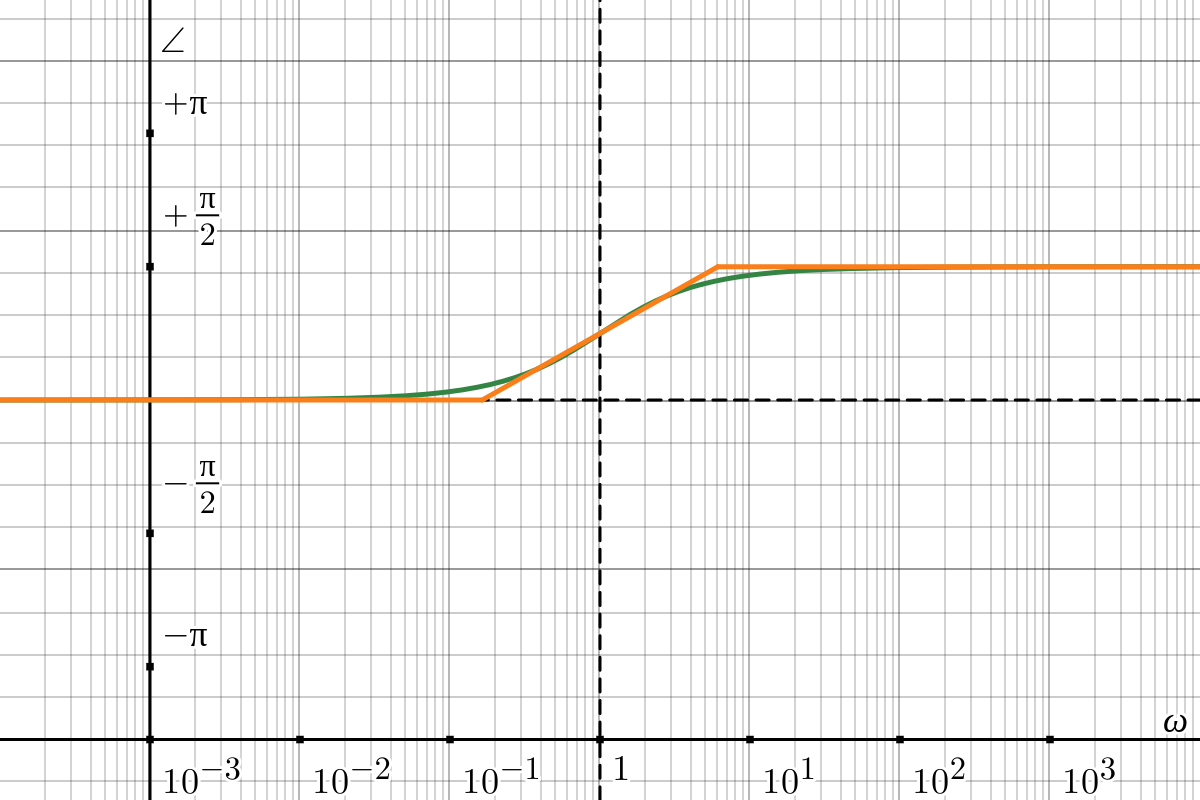
\includegraphics[scale=0.3]{../figures/lowpass_bode/phase_weird.png}
\end{center}
\end{minipage}

\par\medskip

Chiaramente questa è solo un ipotesi in dominio frequenza, trascurando i transienti, e non è il comportamento effettivo che otterremo dal sistema.

\subsubsection{Filtri passa-basso}
I sistemi visti finora rappresentano effettivamente una classe di \textbf{filtri}, detti filtri \textbf{passa-basso}, in quanto lasciano passare solo le frequenze sotto una certa soglia, detta \textbf{frequenza di taglio}.
Al di sotto della frequenza di taglio il segnale resta pressoché invariato, mentre al sopra della frequenza di taglio decade con abbattimento di 6 dB/oct.
Questo chiaramente comporta uno scostamento di fase che va fino a un massimo di $-\frac{\pi}{2}$ dalla fase originale, al di sopra della frequenza di taglio.

Possiamo ottenere abbattimenti più "ripidi", come abbiamo visto, sovrapponendo più filtri.
La loro risposta complessiva sarà infati data da:
$$
G_{eq} = G_1(s) \cdot G_2(s) \cdot ...
$$
che in modulo logaritmico diventa una somma, ergo se l'abbattimento per un singolo filtro è di 6 dB/oct, mettendo insieme $n$ filtri si ha un abbattimento di $6 \cdot n$ dB/oct.

\par\medskip

\noindent
\begin{minipage}{\textwidth}
Vediamo ad esempio il caso di due filtri, quindi per un abbattimento complessivo di 12 dB/oct:
\begin{center}
	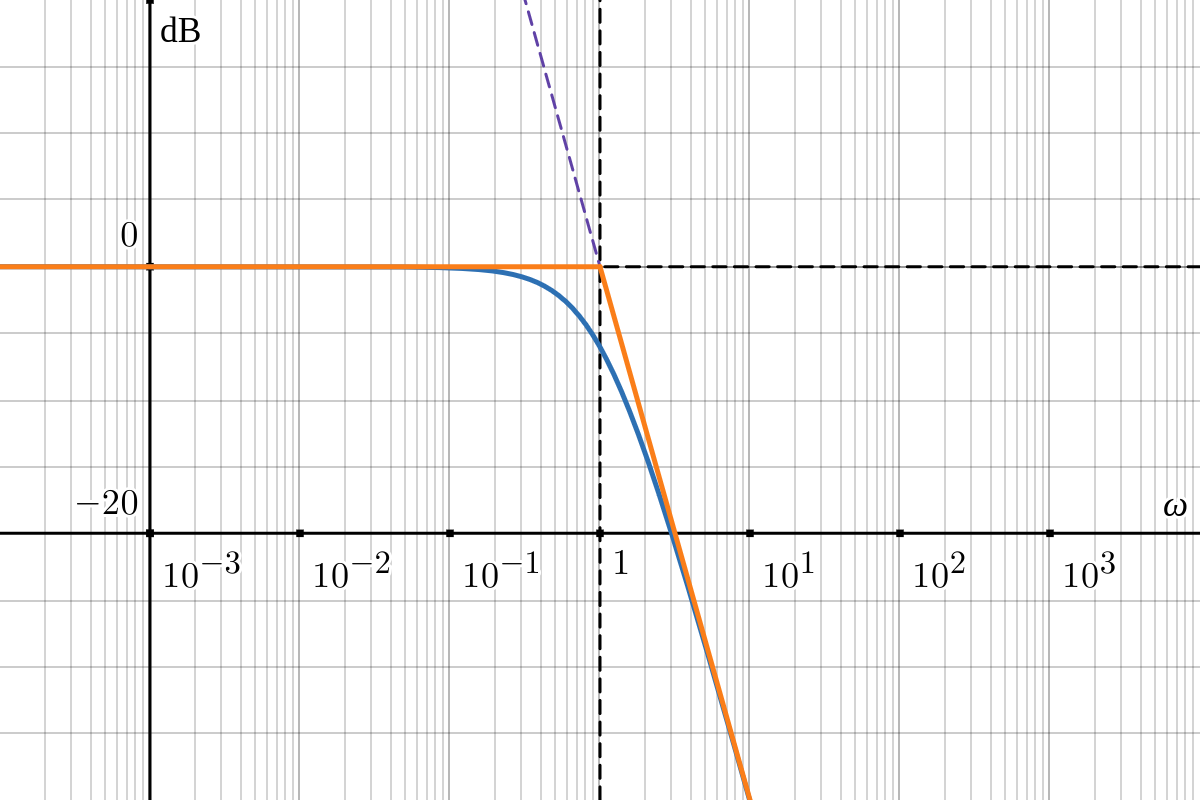
\includegraphics[scale=0.3]{../figures/lowpass_bode/mod_2x.png}
\end{center}
\end{minipage}

\par\bigskip

Dal punto di vista elettronico, un filtro di questo tipo, che viene detto \textbf{filtro passivo}, può essere realizzato come segue:

\begin{center}
	\begin{circuitikz}
		\draw (-4, 1) -- (-3, 1) 
			to [  resistor, l=$R$] (0, 1)
			to [ capacitor, l=$C$] (0, -1) 
			to [ short ] (-3, -1)	
			-- (-4, -1);
			
		\draw (-4.6, 1) node[anchor=west] {$+$};
		\draw (-4.6, 0) node[anchor=west] {$V_1$};
		\draw (-4.6, -1) node[anchor=west] {$-$};

		\draw (4, 1) -- (3, 1) 
			to [short] (0, 1);

		\draw (0, -1) to [ short ] (3, -1)
			-- (4, -1);
	
		\draw (4.6, 1) node[anchor=east] {$+$};
		\draw (4.6, 0) node[anchor=east] {$V_2$};
		\draw (4.6, -1) node[anchor=east] {$-$};
		
	\end{circuitikz}
\end{center}
dove prendiamo $V_1 = u(t)$ come il segnale in entrata, e $V_2 = y(t)$ come il segnale in uscita.

Portandoci nel dominio di Laplace e svolgendo il partitore di tensione, si può quindi ricavare $Y(s)$ da $U(s)$ come:
$$
Y(s) = \frac{ \frac{U(s)}{Cs} }{ R + \frac{1}{Cs} }
$$
e quindi ricavare la funzione di trasferimento:
$$
G(s) = \frac{Y(s)}{U(s)} = \frac{1}{Cs} \cdot \frac{1}{R + \frac{1}{Cs}} = \frac{1}{RCs + 1}
$$
che vediamo non è altro che la forma di Bode della forma studiata finora, con $\tau = RC$ tempo caratteristico.

\subsection{Zeri reali: derivatori}
Vediamo la classe di risposte in frequenza in qualche modo duale a quella degli integratori.

\subsubsection{Zeri all'origine} 
Ricordiamo che lo zero all'origine rappresenta nel dominio di Laplace il \textbf{derivatore}:
$$
s
$$
Considereremo quindi funzioni di trasferimento del tipo:
$$
G(s) = s \implies G(j \omega) = j \omega
$$
passando alla risposta armonica.

Il modulo in questo caso sarà:
$$
|G(j \omega)| = \omega
$$
che notiamo in logaritmo (dB) dà:
$$
20 \log_{10} \left( \omega^{-1} \right) = 20 \log_{10} (\omega)
$$

\par\medskip

\noindent
\begin{minipage}{\textwidth}
cioè si ottiene una retta nel diagramma del modulo logaritmico che passa per $\omega =1$ con modulo 0 dB e pendenza 20 dB/dec (cioè 6 dB/oct):
\begin{center}
	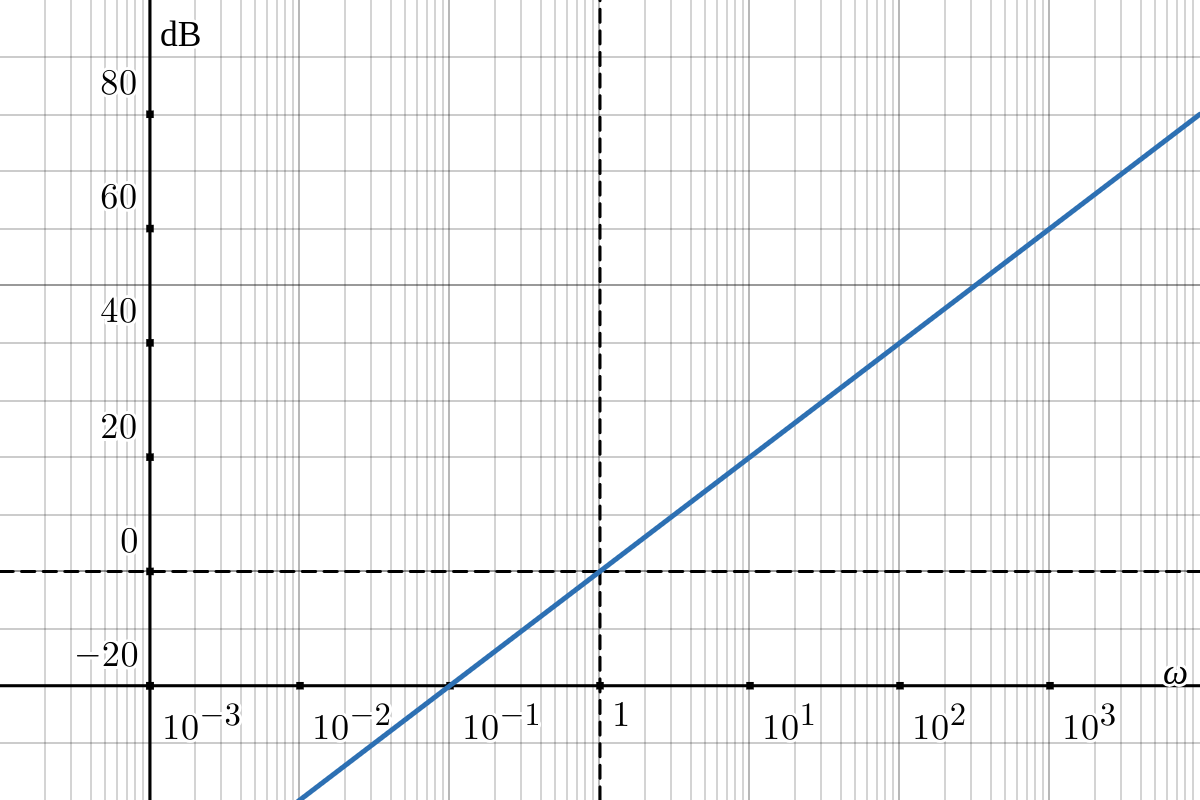
\includegraphics[scale=0.3]{../figures/differentiator_bode/mod.png}
\end{center}
\end{minipage}

\par\medskip

Per quanto riguarda la fase, invece, avremo scostamento costante:
$$
\angle G(j \omega) =  \frac{\pi}{2}
$$

\par\medskip

\noindent
\begin{minipage}{\textwidth}
da cui il grafico:
\begin{center}
	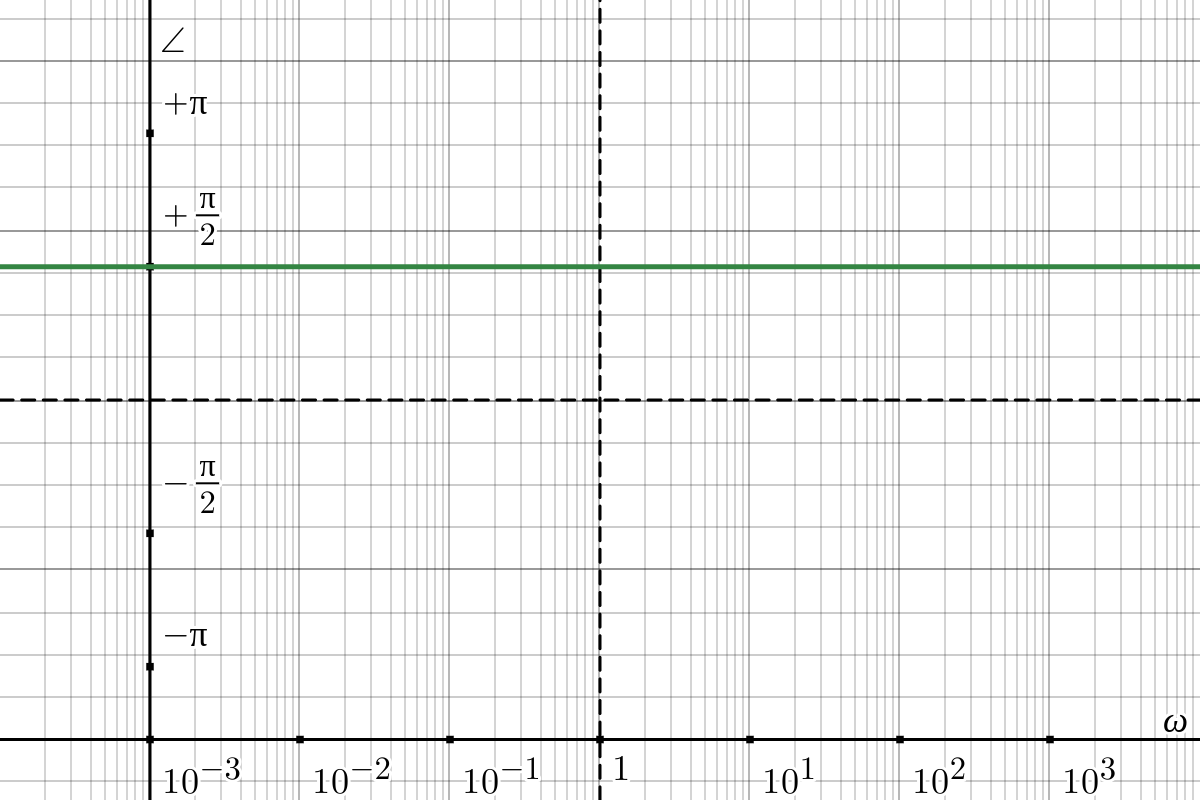
\includegraphics[scale=0.3]{../figures/differentiator_bode/phase.png}
\end{center}
\end{minipage}

\par\medskip

\subsubsection{Zeri reali}
Prendiamo quindi la funzione con un solo zero reale in $-\frac{1}{\tau}$, anche stavolta sovraimponendo alla funzione reale:
$$
G(s) = 1 + s \tau
$$
da cui la risposta armonica:
$$
G(j \omega) = 1 + j \omega \tau
$$

Il modulo è quindi:
$$
|G(j \omega)| = \sqrt{1 + \omega^2 \tau^2}
$$

Vediamo di trovarne un approssimazione \textit{per rette}.
Distinguiamo le situazioni attorno al punto critico, cioè il punto $\omega = 1$:
\begin{itemize}
	\item $\omega^2 \tau^2 << 1$, si ha:
		$$
		|G(j\omega)|_{dB} \approx 0 \, \mathrm{dB}
		$$
		cioè una costante a 0 dB di guadagno;
	\item $\omega^2 \tau^2 << 1$, si ha, trascurando $1$:
		$$
		|G(j \omega)|_{dB} = 20 \log_{10} \left( \omega \tau \right) =
		20 \log \left( \tau \right) + 20 \log \left( \omega \right)
		$$
		che per $\tau = 1$ dà una retta con pendenza 20 dB/dec (cioè -6 db/oct).
\end{itemize}

\par\medskip

\noindent
\begin{minipage}{\textwidth}
Tracciamo quindi il grafico approssimato (sotto al quale si è tracciato il grafico esatto):
\begin{center}
	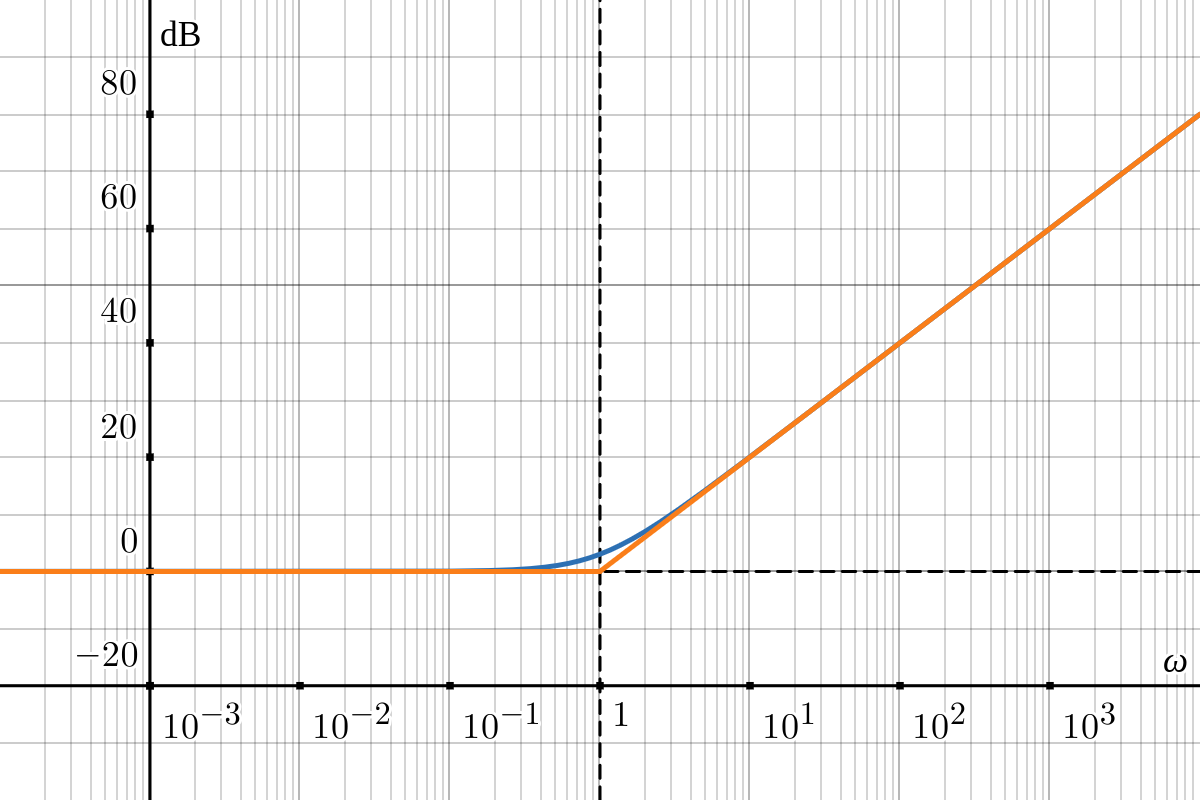
\includegraphics[scale=0.3]{../figures/rdifferentiator_bode/mod.png} 
\end{center}
\end{minipage}

\par\medskip

La fase è invece:
$$
\angle G(j \omega) = \tan^{-1} (\omega \tau)
$$

che potremo approssimare in:
\[
	\begin{cases}
		w \tau << 1 \implies \angle G(j\omega) \approx 0^\circ \\ 	
		w \tau >> 1 \implies \angle G(j\omega) \approx 90^\circ \\ 	
		w \tau = 1 \implies \angle G(j\omega) = 45^\circ \\ 	
	\end{cases}
\]
preso $\tau > 0$.

\par\medskip

\noindent
\begin{minipage}{\textwidth}
Approssimiamo quindi questa funzione prendendo le rette a $0^\circ$ e $90^\circ$, interpolate da una retta passante da $45^\circ$ a $\omega = 1$:
\begin{center}
	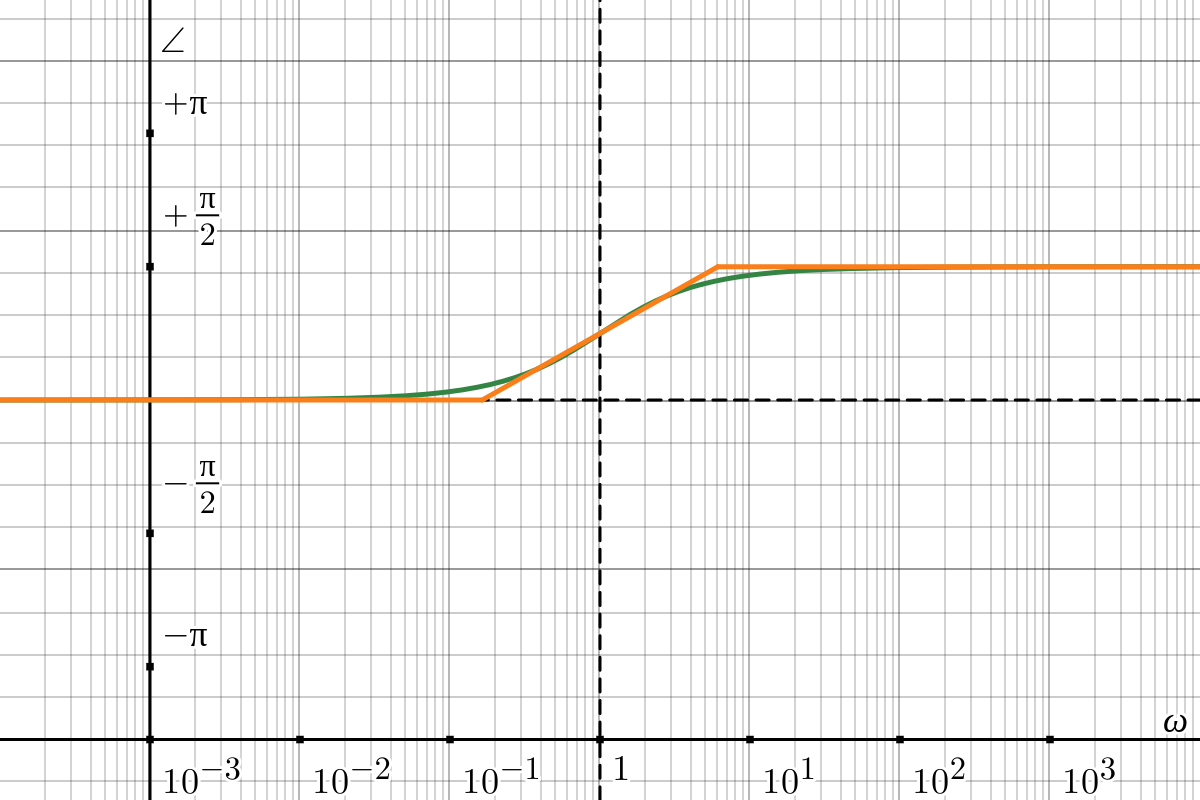
\includegraphics[scale=0.3]{../figures/rdifferentiator_bode/phase.png}
\end{center}
\end{minipage}

\par\medskip

Notiamo quindi che valgono tutte le considerazioni fatte sugli integratori reali, cioè capovolgendo lo zero si trova scostamento in fase opposto, ecc...

\subsection{Poli multipli}
Possiamo sfruttare la proprietà di trasformazione in somma del prodotto logaritmico per tracciare i diagrammi di Bode di funzioni di trasferimento con poli doppi.

Prendiamo ad esempio: 
$$
G(s) = \frac{1}{(1 + s)^2}
$$
che dà la risposta armonica:
$$
G(j \omega) = \frac{1}{(1 + j \omega)^2}
$$

Questo non è altro che il prodotto di due poli semplici:
$$
G(j \omega) = \frac{1}{1 + j \omega^2} \cdot \frac{1}{1 + j \omega^2}
$$
cioè sommiamo moduli e fasi, ottenendo un decadimento di 40 dB/dec e uno scostamento di fase massimo di $-180^\circ$.

Generalizzando a poli multipli, si ha semplicemente:
$$
G(s) = \frac{1}{(1 + s)^n} \implies G(j \omega) = \frac{1}{(1 + j \omega)^n} = \frac{1}{1 + j \omega^2} \cdot \frac{1}{1 + j \omega^2} \cdot ...
$$
cioè si continuano a sommare moduli e fasi, ottenendo decadimenti di $n \cdot 20 $ db/dec e scostamenti di fase massimi di $n \cdot -90^\circ$.

Notiamo che questo non è altro che il comportamento che avevamo descritto studiando filtri sovrapposti, per abbattimenti più ripidi, ad esempio in 17.3.3.

\end{document}
